\documentclass[11pt]{article}

\usepackage{ulem}
\usepackage{tikz}
\usepackage{xurl}
\usepackage{float}
\usepackage{amsmath}
\usepackage{booktabs}
\usepackage{graphicx}
\usepackage{listings}
\usepackage[T5]{fontenc}
\usepackage{indentfirst}
\usepackage[utf8]{inputenc}
\usepackage[margin=1in]{geometry}
\usetikzlibrary{arrows.meta, positioning}

\begin{document}

\begin{center}

{\Large \textbf{UNIVERSITY OF SCIENCE AND TECHNOLOGY OF HANOI}}\\
\vspace{0.3cm}
----------------------o0o----------------------\\

\vspace{4cm}

{\large
\centerline{2540027 - Nguyễn Xuân Vinh}
}

\vspace{4cm}

{\Huge \textbf{BC3.04a Advanced Programming for HPC}}\\
\vspace{0.5cm}
Lecturer: Dr. Trần Giang Sơn

\vspace{4cm}

{\Large \textbf{REPORT LABWORK 8}}\\

\vspace{0.5cm}

{\large
Subjects: Scatter
}

\vspace{4cm}
\today
\end{center}

\newpage

\newpage

\tableofcontents

\newpage

\section{Objective}

The objective of the labwork 8 is to prepare the image data representation for the next Gather labwork. The input image is converted from RGB to HSV and from an Array of Structures (AoS) representation to a Structure of Arrays (SoA) representation.

The implemented operations are:

\begin{itemize}
\item Convert RGB AoS to HSV SoA.
\item Convert HSV SoA back to RGB AoS.
\item Implement the two 2D scatter kernels \texttt{RGB2HSV()} and \texttt{HSV2RGB()}.
\item Test the round-trip conversion using a sample image.
\item Compare the reconstructed RGB image with the original image.
\item Measure the execution time using different 2D block sizes.
\end{itemize}

\section{Input Image and Data Representation}

The input image was loaded from \texttt{/content/img.jpg} using OpenCV. OpenCV initially loads an image in BGR format, so it was converted to RGB before applying the implemented kernels.

The input image has the following dimensions:

$$
1920 \times 1080 \times 3
$$

The RGB image uses an AoS representation, where each pixel contains three components:

$$
[R,G,B]
$$

Therefore, the image can be represented as:

$$
[R,G,B]\ [R,G,B]\ [R,G,B]\ \ldots
$$

For HSV, the data is converted to an SoA representation consisting of three separate arrays:

$$
H[],\quad S[],\quad V[]
$$

The three arrays contain the Hue, Saturation, and Value components of the image.

\section{RGB to HSV -- \texttt{RGB2HSV()}}

The first scatter kernel is \texttt{RGB2HSV()}. It converts RGB AoS data into three separate HSV arrays.

The RGB values are first scaled from the range $[0,255]$ to $[0,1]$:

$$
R'=\frac{R}{255},\qquad
G'=\frac{G}{255},\qquad
B'=\frac{B}{255}
$$

The maximum and minimum values are then calculated:

$$
max=\max(R',G',B')
$$

$$
min=\min(R',G',B')
$$

and:

$$
\Delta=max-min
$$

The Hue value is calculated according to the component having the maximum value:

$$
H=
\begin{cases}
0 & \Delta=0\\
60\left(\frac{G'-B'}{\Delta}\bmod6\right) & max=R'\\
60\left(\frac{B'-R'}{\Delta}+2\right) & max=G'\\
60\left(\frac{R'-G'}{\Delta}+4\right) & max=B'
\end{cases}
$$

The Saturation is calculated as:

$$
S=
\begin{cases}
0 & max=0\\
\frac{\Delta}{max} & max\neq0
\end{cases}
$$

and the Value is:

$$
V=max
$$

The resulting values are stored in three separate arrays $H$, $S$, and $V$.

The kernel processes the image block by block using the selected 2D block size.

\begin{figure}[H]
\centering
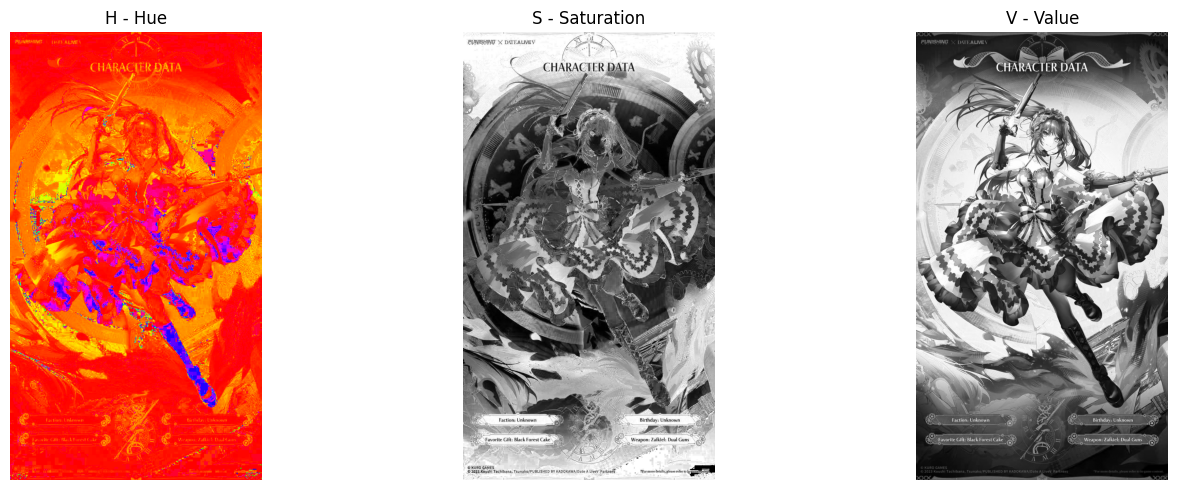
\includegraphics[width=0.95\textwidth]{hsv_components.png}
\caption{H, S, and V components generated by the RGB2HSV kernel.}
\label{fig:hsv_components}
\end{figure}

\section{HSV to RGB -- \texttt{HSV2RGB()}}

The second scatter kernel is \texttt{HSV2RGB()}. It converts the three HSV arrays back into an RGB AoS image.

First, the Hue value is converted using:

$$
d=\frac{H}{60}
$$

$$
h_i=\lfloor d\rfloor\bmod6
$$

$$
f=d-\lfloor d\rfloor
$$

The intermediate values are calculated as:

$$
l=V(1-S)
$$

$$
m=V(1-fS)
$$

$$
n=V(1-(1-f)S)
$$

Depending on the value of $h_i$, the RGB components are calculated using the six cases:

$$
(R,G,B)=
\begin{cases}
(V,n,l) & h_i=0\\
(m,V,l) & h_i=1\\
(l,V,n) & h_i=2\\
(l,m,V) & h_i=3\\
(n,l,V) & h_i=4\\
(V,l,m) & h_i=5
\end{cases}
$$

Finally, the RGB values are scaled from $[0,1]$ to $[0,255]$ and stored as a three-channel RGB image.

The resulting RGB image therefore returns from the SoA representation to the original AoS representation.

\section{Round-trip Test}

The two kernels were tested sequentially:

\begin{center}
RGB\ AoS
$\rightarrow$
RGB2HSV
$\rightarrow$
HSV\ SoA
$\rightarrow$
HSV2RGB
$\rightarrow$
RGB\ AoS
\end{center}

The reconstructed image was compared with the original RGB image using the absolute pixel difference.

For the tested image, the results were:

\begin{itemize}
\item Maximum absolute difference: $1$
\item Mean absolute difference: $0.174219$
\end{itemize}

The maximum difference of one intensity level is caused by floating-point calculation and conversion back to 8-bit integer RGB values.

\begin{figure}[H]
\centering
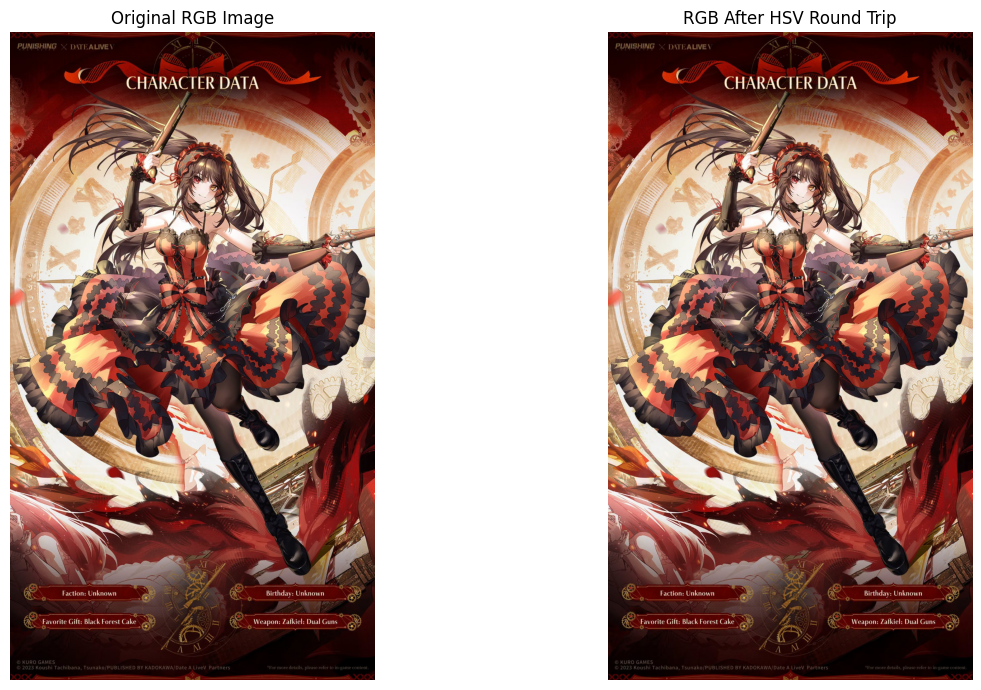
\includegraphics[width=0.95\textwidth]{rgb_round_trip.png}
\caption{Original RGB image and RGB image reconstructed after the HSV round-trip conversion.}
\label{fig:round_trip}
\end{figure}

\section{Experiment with Different 2D Block Sizes}

The two scatter kernels were tested using five different 2D block sizes:

$$
4\times4,\quad
8\times8,\quad
16\times16,\quad
32\times32,\quad
64\times64
$$

For each block size, the execution time of both kernels was measured.

\begin{table}[H]
\centering
\caption{Execution time of the RGB2HSV and HSV2RGB kernels}
\label{tab:benchmark}
\begin{tabular}{ccccc}
\toprule
Block Size & RGB2HSV (s) & HSV2RGB (s) & Total (s) & Max Difference \\
\midrule
$4\times4$   & 7.863127 & 10.186895 & 18.050022 & 1 \\
$8\times8$   & 1.635624 & 2.178716 & 3.814341 & 1 \\
$16\times16$ & 0.503685 & 0.682065 & 1.185750 & 1 \\
$32\times32$ & 0.209837 & 0.264616 & 0.474453 & 1 \\
$64\times64$ & 0.105950 & 0.157785 & 0.263735 & 1 \\
\bottomrule
\end{tabular}
\end{table}

The mean absolute difference was $0.174219$ for all tested block sizes.

A correctness check was also performed by comparing the reconstructed image from each block size with the $16\times16$ reference result.

\begin{table}[H]
\centering
\caption{Correctness verification for different block sizes}
\label{tab:correctness}
\begin{tabular}{cc}
\toprule
Block Size & Identical to $16\times16$ Result \\
\midrule
$4\times4$   & True \\
$8\times8$   & True \\
$16\times16$ & True \\
$32\times32$ & True \\
$64\times64$ & True \\
\bottomrule
\end{tabular}
\end{table}

\begin{figure}[H]
\centering
\includegraphics[width=0.95\textwidth]{figures/block_size_results.png}
\caption{HSV round-trip results using different 2D block sizes.}
\label{fig:block_sizes}
\end{figure}

\section{Performance and Speedup}

The implementation measures the execution time of both scatter kernels for different 2D block sizes.

No separate optimized implementation was used as a baseline. Therefore, a conventional speedup value is not calculated in this labwork. The measured execution times are shown in Table~\ref{tab:benchmark}.

\section{Conclusion}

In the labwork 8, the two required 2D scatter kernels, \texttt{RGB2HSV()} and \texttt{HSV2RGB()}, were implemented.

The RGB input was converted from an AoS representation into three separate HSV arrays $H$, $S$, and $V$. The data was then converted back from the HSV SoA representation into an RGB AoS image.

The round-trip test produced a maximum absolute difference of $1$ and a mean absolute difference of $0.174219$ compared with the original image. The same reconstructed result was obtained for all tested block sizes when compared with the $16\times16$ reference result.

The kernels were also tested using five different 2D block sizes, and their execution times were measured.

\end{document}